\documentclass[10pt,twocolumn]{article}

\usepackage[margin=0.72in]{geometry}
\usepackage{graphicx}
\usepackage{booktabs}
\usepackage{tabularx}
\usepackage{longtable}
\usepackage{xcolor}
\usepackage[hidelinks]{hyperref}
\usepackage{microtype}

\newcommand{\TODO}[1]{\textbf{[TODO: #1]}}
\newcommand{\TODOCITE}[1]{\textbf{[CITATION NEEDED: #1]}}
\newcommand{\TargetedOverall}{0.840868}
\newcommand{\DevelopmentFullOverall}{0.884842}
\newcommand{\DevelopmentRetrievalOverall}{0.563853}
\newcommand{\DevelopmentNoMemoryOverall}{0.366713}
\newcommand{\FormalOverall}{0.866546}
\newcommand{\ComparisonFullOverall}{0.870698}
\newcommand{\ComparisonRetrievalOverall}{0.552346}
\newcommand{\ComparisonNoMemoryOverall}{0.364683}


\title{Omni-Context: Evidence-Linked Manuscript Scaffold}
\author{\TODO{Author names and affiliations required.}}
\date{}

\begin{document}
\maketitle

\begin{abstract}
% CONTENT GOAL: State the system scope, internal evaluation protocol, central verified findings, and limitations in a compact form.
% QUESTIONS FOR AUTHORS: What problem definition and contribution framing should lead? Which verified results belong in the abstract?
% VERIFIED FACT: Internal Development-35 mode scores are exposed through \DevelopmentFullOverall, \DevelopmentRetrievalOverall, and \DevelopmentNoMemoryOverall.
% VERIFIED FACT: Formal-250 is 248/250 with two errors; category-macro Overall is \FormalOverall.
% EVIDENCE: docs/omni-context-paper-evidence-v1/metrics/development-35-summary.json
% EVIDENCE: docs/omni-context-paper-evidence-v1/metrics/formal-250-summary.json
% ALLOWED: Clearly bounded internal Synthetic Curated Benchmark claims.
% FORBIDDEN: Universal SOTA, external validity, Formal 250/250, or completed LoCoMo claims.
\TODO{Author prose required.}
\end{abstract}

\section{Introduction}
% CONTENT GOAL: Motivate evidence-grounded long-term memory and state the paper's contributions without exceeding verified evidence.
% QUESTIONS FOR AUTHORS: What user/system failure motivates Omni-Context? Which contributions are product mechanisms versus evaluation assets?
% VERIFIED FACT: The frozen product separates ingestion, memory storage, multi-channel retrieval, fusion, reranking, evidence grouping, evidence selection, and provenance output.
% EVIDENCE: docs/omni-context-paper-evidence-v1/architecture/module-to-code-map.csv
% CITATION PLACEHOLDER: literature motivation must be supplied and verified by the authors.
\TODOCITE{long-term memory for language agents}
\TODO{Author prose required.}

\section{Related Work}
% CONTENT GOAL: Position the system relative to verified literature supplied later by the research lead.
% QUESTIONS FOR AUTHORS: Which memory architectures, retrieval systems, temporal knowledge methods, and agent benchmarks are relevant?
% REFERENCE RULE: Do not create citation keys until the corresponding bibliographic records are verified.
\TODOCITE{retrieval-augmented generation and agent memory}
\TODOCITE{temporal knowledge representation}
\TODOCITE{evaluation of long-horizon language agents}
\TODO{Author prose required after literature verification.}

\section{Method}
% CONTENT GOAL: Describe the frozen product pipeline and the Candidate v3.1 evidence-selection fix at code-verifiable granularity.
% QUESTIONS FOR AUTHORS: Which data structures and interfaces require formal notation? Which implementation details belong in the appendix?
% VERIFIED FACT: Retrieval uses text, vector, assertion, graph, and subject-attachment channels before source-aware fusion and query-aware evidence selection.
% VERIFIED FACT: Benchmark Gold never enters the product retrieval path.
% EVIDENCE: docs/omni-context-paper-evidence-v1/architecture/final-product-fix.md
% EVIDENCE: docs/omni-context-paper-evidence-v1/architecture/module-to-code-map.csv
% ALLOWED: Describe the frozen implementation and its verified internal preflight behavior.
% FORBIDDEN: Claim that the fix universally improves retrieval.

\begin{figure*}[t]
  \centering
  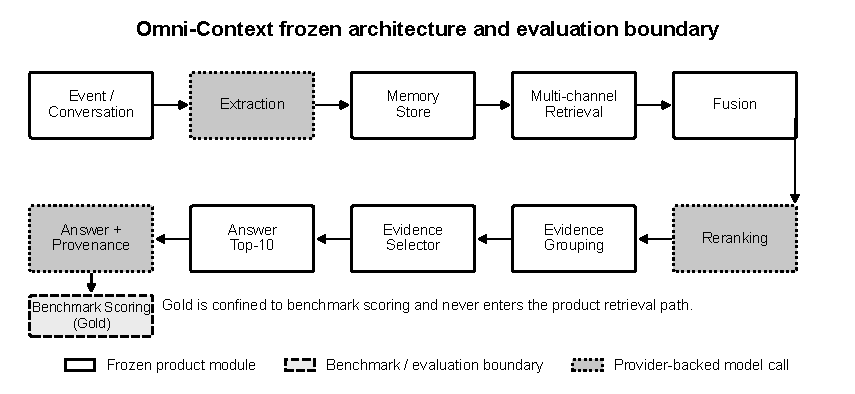
\includegraphics[width=\textwidth]{../figures/architecture.pdf}
  \caption{Frozen product architecture and evaluation boundary. Product modules, benchmark boundaries, and provider-backed calls use distinct line/fill styles.}
  \label{fig:architecture}
\end{figure*}

\begin{figure*}[t]
  \centering
  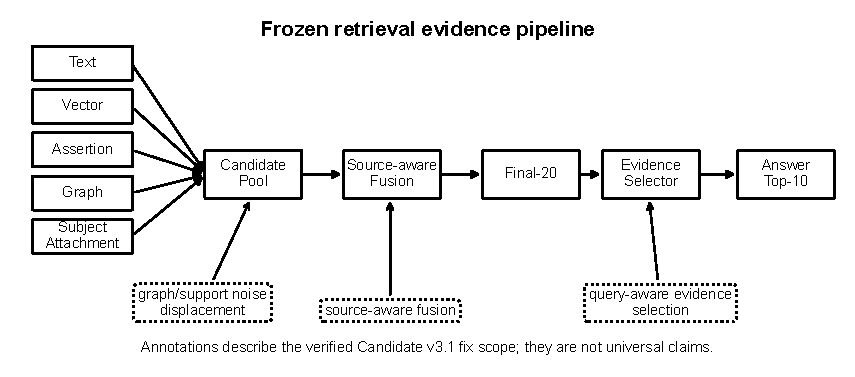
\includegraphics[width=\textwidth]{../figures/retrieval-pipeline.pdf}
  \caption{Evidence retrieval pipeline and the bounded scope of the final Candidate v3.1 fix.}
  \label{fig:retrieval-pipeline}
\end{figure*}

\TODO{Author prose required.}

\section{Benchmark}
% CONTENT GOAL: Define the seven categories, splits, mode comparisons, scoring aggregation, and dataset scope.
% QUESTIONS FOR AUTHORS: How were scenarios constructed? Which validity arguments can be supported without held-out results?
% VERIFIED FACT: Seven capability categories are reported using the benchmark's category-macro definition.
% VERIFIED FACT: The reported evaluations primarily use the internal Synthetic Curated Benchmark.
% VERIFIED FACT: LoCoMo is NOT RUN; Candidate v3.1 was not bound to the existing held-out authorization.
% EVIDENCE: docs/omni-context-paper-evidence-v1/metrics/formal-250-by-category.csv
% EVIDENCE: docs/omni-context-paper-evidence-v1/reproducibility/known-limitations.md
% FORBIDDEN: Treat category-macro results as scenario-weighted means or claim external held-out validation.
\TODO{Author prose required.}

\section{Experimental Setup}
% CONTENT GOAL: State version locks, runtime attestation, model configuration, isolation, retries, checkpointing, and scoring verification.
% QUESTIONS FOR AUTHORS: Which hardware details are publication-relevant? How should provider dependence be disclosed?
% VERIFIED FACT: Product commit 17dc1d0107b0474de84058205a91b302ba290a74 and benchmark commit 62b0b20f944f7e9a2c58f02ce1c65bb43dfbf841 are frozen.
% VERIFIED FACT: 105 deterministic rescore records produced zero scoring differences and zero scoring defects.
% EVIDENCE: docs/omni-context-paper-evidence-v1/manifests/reproducibility-lock.json
% EVIDENCE: docs/omni-context-paper-evidence-v1/metrics/headline-metrics.json
\begin{table*}[t]
\centering\small
\caption{Version and reproducibility locks.}
\label{tab:reproducibility}
\begin{tabular}{lp{0.73\textwidth}}
\toprule Item & Locked value \\
\midrule
Product commit & \texttt{17dc1d0107b0474de84058205a91b302ba290a74} \\
Benchmark commit & \texttt{62b0b20f944f7e9a2c58f02ce1c65bb43dfbf841} \\
Evidence commit & \texttt{ad1fe8806255e420e65398ae67df0a50474356d4} \\
Embedding & Xenova/multilingual-e5-large, revision \texttt{a19b072cb4f0cc8bf98b4e46f90a787a61380979}, 1024 dimensions \\
Answer & deepseek-v4-flash, max tokens 1200, temperature 0, thinking disabled \\
Deterministic rescore & 105 records, 0 differences, 0 scoring defects \\
Open issues & P0=0; P1 classes=2 \\
LoCoMo & NOT RUN; Conversation 2--10 accessed=false \\
\bottomrule
\end{tabular}
\end{table*}

\TODO{Author prose required.}

\section{Results}
% CONTENT GOAL: Report all completed/error counts next to category-macro scores and keep internal mode comparisons bounded.
% VERIFIED FACT: Development Full Omni=\DevelopmentFullOverall, Retrieval-only=\DevelopmentRetrievalOverall, No Memory=\DevelopmentNoMemoryOverall.
% VERIFIED FACT: Formal completed 248/250 with two errors and Overall=\FormalOverall.
% VERIFIED FACT: Comparison Full Omni=\ComparisonFullOverall; Retrieval-only is 69/70 at \ComparisonRetrievalOverall; No Memory=\ComparisonNoMemoryOverall.
% EVIDENCE: docs/omni-context-paper-evidence-v1/metrics/
% FORBIDDEN: Call the mode comparison a strict component ablation.

\begin{table*}[t]
\centering
\caption{Version-locked internal benchmark results. Completed and error counts are never suppressed.}
\label{tab:main-results}
\begin{tabular}{llrrr}
\toprule
Evaluation & Mode & Completed & Errors & Overall \\
\midrule
Targeted-7 & Full Omni & 7/7 & 0 & 0.840868 \\
Development-35 & Full Omni & 35/35 & 0 & 0.884842 \\
Development-35 & Retrieval-only & 35/35 & 0 & 0.563853 \\
Development-35 & No Memory & 35/35 & 0 & 0.366713 \\
Formal-250 & Full Omni & 248/250 & 2 & 0.866546 \\
Comparison-70 & Full Omni & 70/70 & 0 & 0.870698 \\
Comparison-70 & Retrieval-only & 69/70 & 1 & 0.552346 \\
Comparison-70 & No Memory & 70/70 & 0 & 0.364683 \\
\bottomrule
\end{tabular}
\begin{minipage}{0.96\textwidth}\footnotesize
Formal-250 Overall is computed over successfully completed records using the benchmark's category-macro definition. These mode comparisons are not strict component ablations. All evaluations shown here are internal Synthetic Curated Benchmark results; external held-out validity has not been established.
\end{minipage}
\end{table*}

\begin{table*}[t]
\centering\small
\caption{Category-macro results. The mode delta is Comparison-70 Full Omni minus the stronger of Retrieval-only and No Memory.}
\label{tab:category-results}
\begin{tabular}{lrrrrrr}
\toprule
Category & Dev Full & Formal Full & Comp Full & Comp Ret. & Comp No Mem. & $\Delta$ \\
\midrule
Cognitive Continuity & 0.916667 & 0.936667 & 0.956667 & 0.616667 & 0.500000 & 0.340000 \\
Memory Evolution & 0.856746 & 0.852866 & 0.897963 & 0.407130 & 0.208333 & 0.490833 \\
Conflict Resolution & 0.833333 & 0.812500 & 0.788889 & 0.327160 & 0.222222 & 0.461729 \\
Cross-Agent Transfer & 1.000000 & 1.000000 & 0.994444 & 0.755556 & 0.500000 & 0.238888 \\
Human-like Forgetting & 0.927778 & 0.884722 & 0.886111 & 0.669444 & 0.416667 & 0.216667 \\
Proactive Insight & 0.875000 & 0.770833 & 0.800000 & 0.487500 & 0.400000 & 0.312500 \\
Decision Quality & 0.784370 & 0.808235 & 0.770815 & 0.602963 & 0.305556 & 0.167852 \\
\bottomrule
\end{tabular}
\begin{minipage}{0.98\textwidth}\footnotesize
Values are benchmark category means, not scenario-weighted averages. Development and Formal baseline-by-category values are not invented; only available verified columns are shown.
\end{minipage}
\end{table*}


\begin{figure}[t]
  \centering
  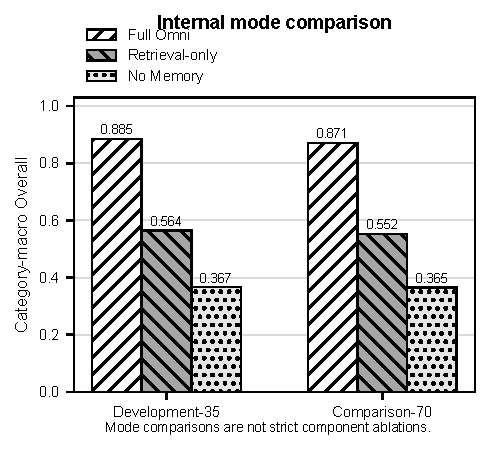
\includegraphics[width=\columnwidth]{../figures/overall-comparison.pdf}
  \caption{Internal Development-35 and Comparison-70 mode results.}
  \label{fig:overall-comparison}
\end{figure}

\begin{figure*}[t]
  \centering
  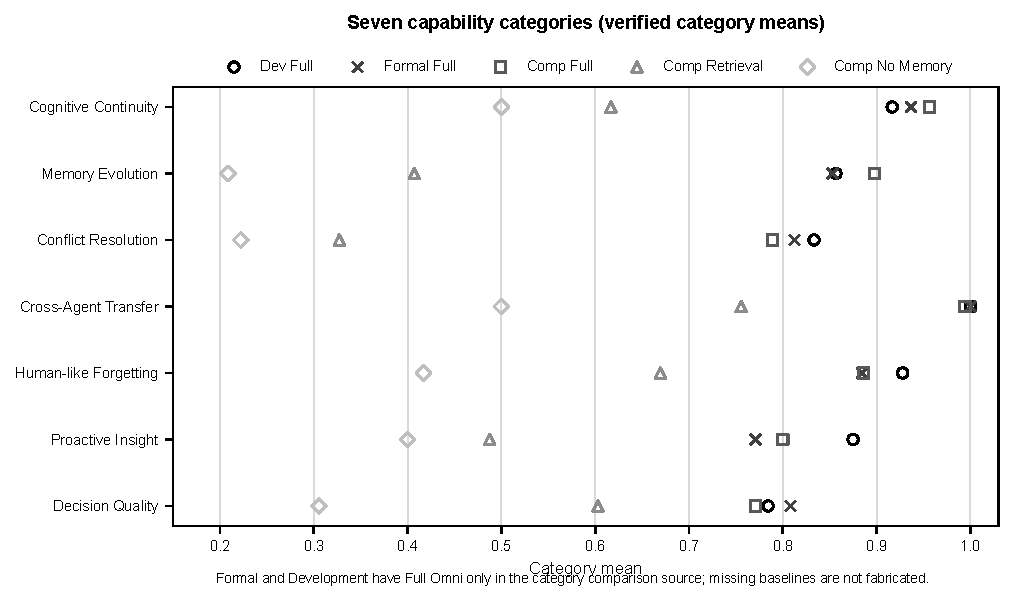
\includegraphics[width=\textwidth]{../figures/category-comparison.pdf}
  \caption{Verified category means. Missing Development/Formal baselines are not fabricated.}
  \label{fig:category-comparison}
\end{figure*}

\TODO{Author interpretation required.}

\begin{table*}[t]
\centering\small
\caption{External held-out evaluation status. No score is available or implied.}
\label{tab:external-heldout}
\begin{tabularx}{\textwidth}{p{0.20\textwidth}p{0.20\textwidth}X p{0.10\textwidth}}
\toprule
Benchmark & Adapter fixtures & Preregistration & Formal result \\
\midrule
LongMemEval-S cleaned & PASS (12 fictional records) & Adapter locked; dataset authorization pending & \textbf{NOT RUN} \\
LoCoMo QA, Conversations 2--10 & PASS (4 fictional QA forms) & Adapter locked; dataset authorization pending & \textbf{NOT RUN} \\
\bottomrule
\end{tabularx}
\end{table*}


\section{Analysis}
% CONTENT GOAL: Analyze retrieval coverage, final product fix evidence, efficiency, and retained failure modes.
% QUESTIONS FOR AUTHORS: Which causal interpretations are supported by the fix diff and preflight? Which remain hypotheses?
% VERIFIED FACT: Retrieval-preflight Top-10 slot coverage changed from 20/38 to 37/38 across the documented general fix.
% VERIFIED FACT: Targeted Candidate Pool, Final-20, and Answer Top-10 each covered 28/30 slots under a different statistical denominator.
% EVIDENCE: docs/omni-context-paper-evidence-v1/architecture/final-product-fix.md
% EVIDENCE: docs/omni-context-paper-evidence-v1/metrics/targeted-7-summary.json

\begin{figure*}[t]
  \centering
  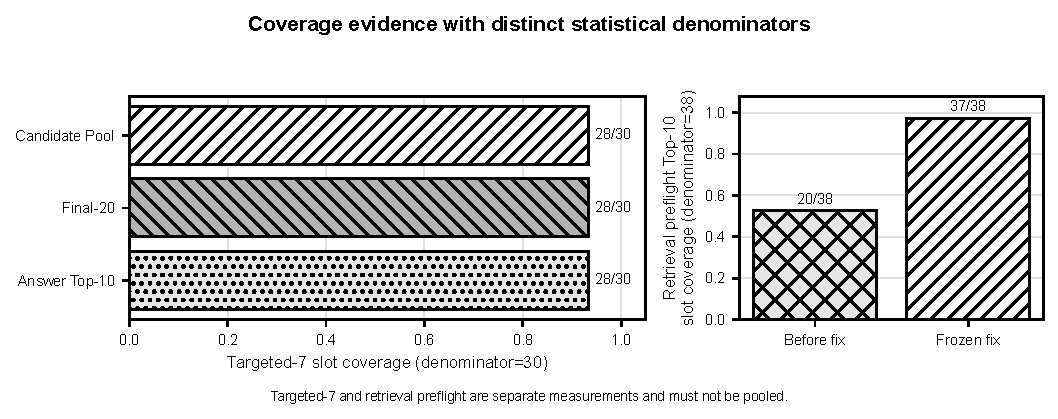
\includegraphics[width=\textwidth]{../figures/coverage-funnel.pdf}
  \caption{Coverage evidence with Targeted and retrieval-preflight denominators kept separate.}
  \label{fig:coverage}
\end{figure*}

\begin{figure*}[t]
  \centering
  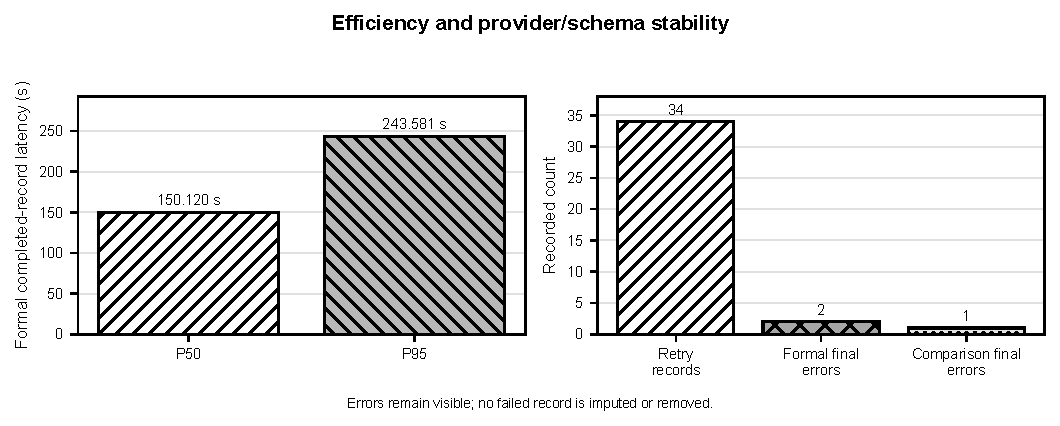
\includegraphics[width=\textwidth]{../figures/latency-summary.pdf}
  \caption{Formal latency and retained retry/error counts.}
  \label{fig:efficiency}
\end{figure*}

\begin{table}[t]
\centering
\caption{Efficiency and stability facts retained without error smoothing.}
\label{tab:efficiency}
\begin{tabular}{lr}
\toprule Metric & Value \\
\midrule
Formal latency P50 & 150120 ms \\
Formal latency P95 & 243581 ms \\
Retry records & 34 \\
Formal final errors & 2 \\
Comparison final errors & 1 \\
\bottomrule
\end{tabular}
\end{table}

\begin{table*}[t]
\centering\scriptsize
\caption{Terminal errors retained after three prescribed attempts. No failed record entered score aggregation.}
\label{tab:errors}
\begin{tabular}{p{0.20\textwidth}lllclclp{0.18\textwidth}p{0.20\textwidth}}
\toprule Scenario & Eval. & Mode & Error & Attempts & Finish & Scored & Attribution & Paper reporting \\
\midrule
\texttt{\detokenize{formal-v2-memory_evolution-039}} & Formal-250 & Full Omni & JSON truncation & 3 & length/length/length & No & Provider structured-output truncation & Retained terminal error; no score imputed \\
\texttt{\detokenize{formal-v2-memory_evolution-040}} & Formal-250 & Full Omni & JSON truncation & 3 & length/length/length & No & Provider structured-output truncation & Retained terminal error; no score imputed \\
\texttt{\detokenize{formal-v2-conflict_resolution-014}} & Comparison-70 & Retrieval-only & empty source\_ids & 3 & stop/stop/stop & No & Baseline schema robustness & Retained terminal error; no score imputed \\
\bottomrule
\end{tabular}
\end{table*}

\TODO{Author analysis required.}

\section{Limitations}
% CONTENT GOAL: Preserve all known limitations and define the boundary of defensible claims.
% VERIFIED FACT: Formal retained two Answer JSON truncation errors after three attempts each.
% VERIFIED FACT: Comparison retained one Retrieval-only empty-source-IDs error after three attempts.
% VERIFIED FACT: Selector and Evidence Group ablations were not run because no existing safe switch was available.
% VERIFIED FACT: unresolved P0=0; unresolved P1 includes two classes.
% VERIFIED FACT: LoCoMo is NOT RUN and Conversation 2--10 remained unaccessed.
% VERIFIED FACT: External validity has not been established.
% EVIDENCE: docs/omni-context-paper-evidence-v1/reproducibility/known-limitations.md
% FORBIDDEN: Universal SOTA, strict-ablation, or held-out-validation claims.
\TODO{Author prose required; do not remove any verified limitation above.}

\section{Conclusion}
% CONTENT GOAL: Summarize only contributions and findings supported by the frozen evidence package, then state the held-out validation next step.
% QUESTIONS FOR AUTHORS: Which contribution list best matches the final paper scope? What future work is authorized to mention?
% ALLOWED: Internal benchmark findings, frozen implementation facts, transparent errors, and future held-out evaluation.
% FORBIDDEN: New empirical claims or universal generalization.
\TODO{Author prose required.}


% Detailed evidence tables use longtable and therefore require one-column mode.
\clearpage
\onecolumn
\appendix
\section{Detailed Category Evidence}
\begin{table*}[t]
\centering\scriptsize
\caption{Development, Formal, and Comparison category distributions over completed records.}
\label{tab:category-details}
\begin{tabular}{llrrrrrr}
\toprule
Evaluation & Category & Completed & Errors & Median & Min & Max & Std. dev. \\
\midrule
Development Full & Cognitive Continuity & 5/5 & 0 & 1.000 & 0.750 & 1.000 & 0.105 \\
Development Full & Memory Evolution & 5/5 & 0 & 0.812 & 0.736 & 1.000 & 0.120 \\
Development Full & Conflict Resolution & 5/5 & 0 & 0.833 & 0.833 & 0.833 & 0.000 \\
Development Full & Cross-Agent Transfer & 5/5 & 0 & 1.000 & 1.000 & 1.000 & 0.000 \\
Development Full & Human-like Forgetting & 5/5 & 0 & 1.000 & 0.694 & 1.000 & 0.119 \\
Development Full & Proactive Insight & 5/5 & 0 & 0.875 & 0.781 & 0.969 & 0.062 \\
Development Full & Decision Quality & 5/5 & 0 & 0.796 & 0.685 & 0.857 & 0.067 \\
Formal Full & Cognitive Continuity & 40/40 & 0 & 1.000 & 0.633 & 1.000 & 0.108 \\
Formal Full & Memory Evolution & 38/40 & 2 & 0.868 & 0.419 & 1.000 & 0.159 \\
Formal Full & Conflict Resolution & 40/40 & 0 & 0.833 & 0.389 & 0.833 & 0.080 \\
Formal Full & Cross-Agent Transfer & 30/30 & 0 & 1.000 & 1.000 & 1.000 & 0.000 \\
Formal Full & Human-like Forgetting & 40/40 & 0 & 0.861 & 0.556 & 1.000 & 0.120 \\
Formal Full & Proactive Insight & 30/30 & 0 & 0.797 & 0.344 & 1.000 & 0.132 \\
Formal Full & Decision Quality & 30/30 & 0 & 0.815 & 0.602 & 0.926 & 0.067 \\
Comparison Full & Cognitive Continuity & 10/10 & 0 & 1.000 & 0.750 & 1.000 & 0.080 \\
Comparison Full & Memory Evolution & 10/10 & 0 & 1.000 & 0.631 & 1.000 & 0.133 \\
Comparison Full & Conflict Resolution & 10/10 & 0 & 0.833 & 0.389 & 0.833 & 0.133 \\
Comparison Full & Cross-Agent Transfer & 10/10 & 0 & 1.000 & 0.944 & 1.000 & 0.017 \\
Comparison Full & Human-like Forgetting & 10/10 & 0 & 0.972 & 0.556 & 1.000 & 0.148 \\
Comparison Full & Proactive Insight & 10/10 & 0 & 0.781 & 0.688 & 0.938 & 0.104 \\
Comparison Full & Decision Quality & 10/10 & 0 & 0.787 & 0.537 & 0.880 & 0.102 \\
Comparison Retrieval & Cognitive Continuity & 10/10 & 0 & 0.617 & 0.550 & 0.733 & 0.049 \\
Comparison Retrieval & Memory Evolution & 10/10 & 0 & 0.384 & 0.208 & 0.648 & 0.201 \\
Comparison Retrieval & Conflict Resolution & 9/10 & 1 & 0.222 & 0.222 & 0.611 & 0.160 \\
Comparison Retrieval & Cross-Agent Transfer & 10/10 & 0 & 0.722 & 0.667 & 0.944 & 0.103 \\
Comparison Retrieval & Human-like Forgetting & 10/10 & 0 & 0.764 & 0.417 & 1.000 & 0.217 \\
Comparison Retrieval & Proactive Insight & 10/10 & 0 & 0.484 & 0.281 & 0.812 & 0.150 \\
Comparison Retrieval & Decision Quality & 10/10 & 0 & 0.606 & 0.481 & 0.727 & 0.078 \\
Comparison No Memory & Cognitive Continuity & 10/10 & 0 & 0.500 & 0.500 & 0.500 & 0.000 \\
Comparison No Memory & Memory Evolution & 10/10 & 0 & 0.208 & 0.208 & 0.208 & 0.000 \\
Comparison No Memory & Conflict Resolution & 10/10 & 0 & 0.222 & 0.222 & 0.222 & 0.000 \\
Comparison No Memory & Cross-Agent Transfer & 10/10 & 0 & 0.500 & 0.500 & 0.500 & 0.000 \\
Comparison No Memory & Human-like Forgetting & 10/10 & 0 & 0.417 & 0.417 & 0.417 & 0.000 \\
Comparison No Memory & Proactive Insight & 10/10 & 0 & 0.406 & 0.375 & 0.438 & 0.023 \\
Comparison No Memory & Decision Quality & 10/10 & 0 & 0.306 & 0.231 & 0.417 & 0.051 \\
\bottomrule
\end{tabular}
\end{table*}

\begin{longtable}{p{0.12\textwidth}p{0.20\textwidth}p{0.60\textwidth}}
\caption{Verified category submetrics.}\label{tab:category-submetrics}\\
\toprule Evaluation & Category & Submetrics \\ \midrule
\endfirsthead
\toprule Evaluation & Category & Submetrics \\ \midrule
\endhead
Development Full & Cognitive Continuity & profile recall=1.000; profile consistency=1.000; constraint utilization=0.667; personalization accuracy=0.833; contradiction rate=0.000; unsupported personalization rate=0.000 \\
Development Full & Memory Evolution & current state accuracy=1.000; historical state preservation=1.000; temporal ordering accuracy=0.457; evolution interpretation accuracy=0.819; stale memory leakage=0.000; state transition accuracy=0.864 \\
Development Full & Conflict Resolution & conflict resolution accuracy=1.000; latest valid fact accuracy=1.000; historical query accuracy=1.000; invalidated fact rejection=1.000; conflict disclosure accuracy=0.000; unsupported resolution rate=0.000 \\
Development Full & Cross-Agent Transfer & cross agent recall=1.000; cross agent consistency=1.000; update propagation accuracy=1.000; provenance preservation=1.000; agent isolation error rate=0.000; stale transfer rate=0.000 \\
Development Full & Human-like Forgetting & salient memory retention=1.000; noise suppression=0.933; false forgetting rate=0.000; stale retention rate=0.133; memory precision=0.967; invalidation accuracy=0.800 \\
Development Full & Proactive Insight & insight precision=0.800; insight recall=0.750; blind spot detection rate=0.850; constraint awareness=0.900; actionability=0.750; unsupported claim rate=0.050; redundant insight rate=0.000; overreach rate=0.000 \\
Development Full & Decision Quality & constraint coverage=0.900; goal alignment=0.750; personalization=0.733; option comparison quality=0.900; risk awareness=0.700; actionability=0.800; internal consistency=0.750; unsupported assumption rate=0.150; overall decision quality=0.676 \\
Formal Full & Cognitive Continuity & profile recall=0.930; profile consistency=1.000; constraint utilization=0.817; personalization accuracy=0.873; contradiction rate=0.000; unsupported personalization rate=0.000 \\
Formal Full & Memory Evolution & current state accuracy=0.947; historical state preservation=0.971; temporal ordering accuracy=0.525; evolution interpretation accuracy=0.814; stale memory leakage=0.000; state transition accuracy=0.861 \\
Formal Full & Conflict Resolution & conflict resolution accuracy=0.975; latest valid fact accuracy=0.975; historical query accuracy=0.950; invalidated fact rejection=0.950; conflict disclosure accuracy=0.025; unsupported resolution rate=0.000 \\
Formal Full & Cross-Agent Transfer & cross agent recall=1.000; cross agent consistency=1.000; update propagation accuracy=1.000; provenance preservation=1.000; agent isolation error rate=0.000; stale transfer rate=0.000 \\
Formal Full & Human-like Forgetting & salient memory retention=1.000; noise suppression=0.883; false forgetting rate=0.000; stale retention rate=0.142; memory precision=0.942; invalidation accuracy=0.625 \\
Formal Full & Proactive Insight & insight precision=0.750; insight recall=0.633; blind spot detection rate=0.742; constraint awareness=0.642; actionability=0.675; unsupported claim rate=0.083; redundant insight rate=0.117; overreach rate=0.075 \\
Formal Full & Decision Quality & constraint coverage=0.900; goal alignment=0.800; personalization=0.811; option comparison quality=0.833; risk awareness=0.642; actionability=0.758; internal consistency=0.850; unsupported assumption rate=0.050; overall decision quality=0.730 \\
Comparison Full & Cognitive Continuity & profile recall=0.960; profile consistency=1.000; constraint utilization=0.867; personalization accuracy=0.913; contradiction rate=0.000; unsupported personalization rate=0.000 \\
Comparison Full & Memory Evolution & current state accuracy=1.000; historical state preservation=0.960; temporal ordering accuracy=0.653; evolution interpretation accuracy=0.871; stale memory leakage=0.000; state transition accuracy=0.903 \\
Comparison Full & Conflict Resolution & conflict resolution accuracy=0.933; latest valid fact accuracy=0.900; historical query accuracy=0.900; invalidated fact rejection=0.900; conflict disclosure accuracy=0.100; unsupported resolution rate=0.000 \\
Comparison Full & Cross-Agent Transfer & cross agent recall=1.000; cross agent consistency=1.000; update propagation accuracy=1.000; provenance preservation=0.967; agent isolation error rate=0.000; stale transfer rate=0.000 \\
Comparison Full & Human-like Forgetting & salient memory retention=1.000; noise suppression=0.900; false forgetting rate=0.000; stale retention rate=0.133; memory precision=0.950; invalidation accuracy=0.600 \\
Comparison Full & Proactive Insight & insight precision=0.825; insight recall=0.675; blind spot detection rate=0.800; constraint awareness=0.650; actionability=0.700; unsupported claim rate=0.025; redundant insight rate=0.150; overreach rate=0.075 \\
Comparison Full & Decision Quality & constraint coverage=0.850; goal alignment=0.775; personalization=0.783; option comparison quality=0.775; risk awareness=0.675; actionability=0.725; internal consistency=0.825; unsupported assumption rate=0.150; overall decision quality=0.679 \\
Comparison Retrieval & Cognitive Continuity & profile recall=0.300; profile consistency=1.000; constraint utilization=0.167; personalization accuracy=0.233; contradiction rate=0.000; unsupported personalization rate=0.000 \\
Comparison Retrieval & Memory Evolution & current state accuracy=0.500; historical state preservation=0.220; temporal ordering accuracy=0.033; evolution interpretation accuracy=0.251; stale memory leakage=0.000; state transition accuracy=0.438 \\
Comparison Retrieval & Conflict Resolution & conflict resolution accuracy=0.407; latest valid fact accuracy=0.000; historical query accuracy=0.000; invalidated fact rejection=0.222; conflict disclosure accuracy=0.333; unsupported resolution rate=0.000 \\
Comparison Retrieval & Cross-Agent Transfer & cross agent recall=0.500; cross agent consistency=1.000; update propagation accuracy=0.200; provenance preservation=0.833; agent isolation error rate=0.000; stale transfer rate=0.000 \\
Comparison Retrieval & Human-like Forgetting & salient memory retention=0.600; noise suppression=0.967; false forgetting rate=0.400; stale retention rate=0.033; memory precision=0.783; invalidation accuracy=0.100 \\
Comparison Retrieval & Proactive Insight & insight precision=0.400; insight recall=0.325; blind spot detection rate=0.325; constraint awareness=0.125; actionability=0.400; unsupported claim rate=0.325; redundant insight rate=0.050; overreach rate=0.300 \\
Comparison Retrieval & Decision Quality & constraint coverage=0.850; goal alignment=0.575; personalization=0.667; option comparison quality=0.525; risk awareness=0.425; actionability=0.350; internal consistency=0.750; unsupported assumption rate=0.200; overall decision quality=0.485 \\
Comparison No Memory & Cognitive Continuity & profile recall=0.000; profile consistency=1.000; constraint utilization=0.000; personalization accuracy=0.000; contradiction rate=0.000; unsupported personalization rate=0.000 \\
Comparison No Memory & Memory Evolution & current state accuracy=0.000; historical state preservation=0.000; temporal ordering accuracy=0.000; evolution interpretation accuracy=0.000; stale memory leakage=0.000; state transition accuracy=0.250 \\
Comparison No Memory & Conflict Resolution & conflict resolution accuracy=0.333; latest valid fact accuracy=0.000; historical query accuracy=0.000; invalidated fact rejection=0.000; conflict disclosure accuracy=0.000; unsupported resolution rate=0.000 \\
Comparison No Memory & Cross-Agent Transfer & cross agent recall=0.000; cross agent consistency=1.000; update propagation accuracy=0.000; provenance preservation=0.000; agent isolation error rate=0.000; stale transfer rate=0.000 \\
Comparison No Memory & Human-like Forgetting & salient memory retention=0.000; noise suppression=1.000; false forgetting rate=1.000; stale retention rate=0.000; memory precision=0.500; invalidation accuracy=0.000 \\
Comparison No Memory & Proactive Insight & insight precision=0.000; insight recall=0.000; blind spot detection rate=0.000; constraint awareness=0.100; actionability=0.100; unsupported claim rate=0.000; redundant insight rate=0.000; overreach rate=0.000 \\
Comparison No Memory & Decision Quality & constraint coverage=0.200; goal alignment=0.025; personalization=0.450; option comparison quality=0.000; risk awareness=0.050; actionability=0.175; internal consistency=0.800; unsupported assumption rate=0.000; overall decision quality=0.050 \\
\bottomrule
\end{longtable}


% references.bib is intentionally empty until references are provided and verified.
\bibliographystyle{plain}
\bibliography{references}
\end{document}
